\documentclass[]{article}
\usepackage{lmodern}
\usepackage{amssymb,amsmath}
\usepackage{ifxetex,ifluatex}
\usepackage{fixltx2e} % provides \textsubscript
\ifnum 0\ifxetex 1\fi\ifluatex 1\fi=0 % if pdftex
  \usepackage[T1]{fontenc}
  \usepackage[utf8]{inputenc}
\else % if luatex or xelatex
  \ifxetex
    \usepackage{mathspec}
  \else
    \usepackage{fontspec}
  \fi
  \defaultfontfeatures{Ligatures=TeX,Scale=MatchLowercase}
\fi
% use upquote if available, for straight quotes in verbatim environments
\IfFileExists{upquote.sty}{\usepackage{upquote}}{}
% use microtype if available
\IfFileExists{microtype.sty}{%
\usepackage{microtype}
\UseMicrotypeSet[protrusion]{basicmath} % disable protrusion for tt fonts
}{}
\usepackage[margin=1in]{geometry}
\usepackage{hyperref}
\hypersetup{unicode=true,
            pdftitle={Simulation of pi},
            pdfauthor={Chao XIA},
            pdfborder={0 0 0},
            breaklinks=true}
\urlstyle{same}  % don't use monospace font for urls
\usepackage{color}
\usepackage{fancyvrb}
\newcommand{\VerbBar}{|}
\newcommand{\VERB}{\Verb[commandchars=\\\{\}]}
\DefineVerbatimEnvironment{Highlighting}{Verbatim}{commandchars=\\\{\}}
% Add ',fontsize=\small' for more characters per line
\usepackage{framed}
\definecolor{shadecolor}{RGB}{248,248,248}
\newenvironment{Shaded}{\begin{snugshade}}{\end{snugshade}}
\newcommand{\KeywordTok}[1]{\textcolor[rgb]{0.13,0.29,0.53}{\textbf{#1}}}
\newcommand{\DataTypeTok}[1]{\textcolor[rgb]{0.13,0.29,0.53}{#1}}
\newcommand{\DecValTok}[1]{\textcolor[rgb]{0.00,0.00,0.81}{#1}}
\newcommand{\BaseNTok}[1]{\textcolor[rgb]{0.00,0.00,0.81}{#1}}
\newcommand{\FloatTok}[1]{\textcolor[rgb]{0.00,0.00,0.81}{#1}}
\newcommand{\ConstantTok}[1]{\textcolor[rgb]{0.00,0.00,0.00}{#1}}
\newcommand{\CharTok}[1]{\textcolor[rgb]{0.31,0.60,0.02}{#1}}
\newcommand{\SpecialCharTok}[1]{\textcolor[rgb]{0.00,0.00,0.00}{#1}}
\newcommand{\StringTok}[1]{\textcolor[rgb]{0.31,0.60,0.02}{#1}}
\newcommand{\VerbatimStringTok}[1]{\textcolor[rgb]{0.31,0.60,0.02}{#1}}
\newcommand{\SpecialStringTok}[1]{\textcolor[rgb]{0.31,0.60,0.02}{#1}}
\newcommand{\ImportTok}[1]{#1}
\newcommand{\CommentTok}[1]{\textcolor[rgb]{0.56,0.35,0.01}{\textit{#1}}}
\newcommand{\DocumentationTok}[1]{\textcolor[rgb]{0.56,0.35,0.01}{\textbf{\textit{#1}}}}
\newcommand{\AnnotationTok}[1]{\textcolor[rgb]{0.56,0.35,0.01}{\textbf{\textit{#1}}}}
\newcommand{\CommentVarTok}[1]{\textcolor[rgb]{0.56,0.35,0.01}{\textbf{\textit{#1}}}}
\newcommand{\OtherTok}[1]{\textcolor[rgb]{0.56,0.35,0.01}{#1}}
\newcommand{\FunctionTok}[1]{\textcolor[rgb]{0.00,0.00,0.00}{#1}}
\newcommand{\VariableTok}[1]{\textcolor[rgb]{0.00,0.00,0.00}{#1}}
\newcommand{\ControlFlowTok}[1]{\textcolor[rgb]{0.13,0.29,0.53}{\textbf{#1}}}
\newcommand{\OperatorTok}[1]{\textcolor[rgb]{0.81,0.36,0.00}{\textbf{#1}}}
\newcommand{\BuiltInTok}[1]{#1}
\newcommand{\ExtensionTok}[1]{#1}
\newcommand{\PreprocessorTok}[1]{\textcolor[rgb]{0.56,0.35,0.01}{\textit{#1}}}
\newcommand{\AttributeTok}[1]{\textcolor[rgb]{0.77,0.63,0.00}{#1}}
\newcommand{\RegionMarkerTok}[1]{#1}
\newcommand{\InformationTok}[1]{\textcolor[rgb]{0.56,0.35,0.01}{\textbf{\textit{#1}}}}
\newcommand{\WarningTok}[1]{\textcolor[rgb]{0.56,0.35,0.01}{\textbf{\textit{#1}}}}
\newcommand{\AlertTok}[1]{\textcolor[rgb]{0.94,0.16,0.16}{#1}}
\newcommand{\ErrorTok}[1]{\textcolor[rgb]{0.64,0.00,0.00}{\textbf{#1}}}
\newcommand{\NormalTok}[1]{#1}
\usepackage{graphicx,grffile}
\makeatletter
\def\maxwidth{\ifdim\Gin@nat@width>\linewidth\linewidth\else\Gin@nat@width\fi}
\def\maxheight{\ifdim\Gin@nat@height>\textheight\textheight\else\Gin@nat@height\fi}
\makeatother
% Scale images if necessary, so that they will not overflow the page
% margins by default, and it is still possible to overwrite the defaults
% using explicit options in \includegraphics[width, height, ...]{}
\setkeys{Gin}{width=\maxwidth,height=\maxheight,keepaspectratio}
\IfFileExists{parskip.sty}{%
\usepackage{parskip}
}{% else
\setlength{\parindent}{0pt}
\setlength{\parskip}{6pt plus 2pt minus 1pt}
}
\setlength{\emergencystretch}{3em}  % prevent overfull lines
\providecommand{\tightlist}{%
  \setlength{\itemsep}{0pt}\setlength{\parskip}{0pt}}
\setcounter{secnumdepth}{0}
% Redefines (sub)paragraphs to behave more like sections
\ifx\paragraph\undefined\else
\let\oldparagraph\paragraph
\renewcommand{\paragraph}[1]{\oldparagraph{#1}\mbox{}}
\fi
\ifx\subparagraph\undefined\else
\let\oldsubparagraph\subparagraph
\renewcommand{\subparagraph}[1]{\oldsubparagraph{#1}\mbox{}}
\fi

%%% Use protect on footnotes to avoid problems with footnotes in titles
\let\rmarkdownfootnote\footnote%
\def\footnote{\protect\rmarkdownfootnote}

%%% Change title format to be more compact
\usepackage{titling}

% Create subtitle command for use in maketitle
\newcommand{\subtitle}[1]{
  \posttitle{
    \begin{center}\large#1\end{center}
    }
}

\setlength{\droptitle}{-2em}

  \title{Simulation of pi}
    \pretitle{\vspace{\droptitle}\centering\huge}
  \posttitle{\par}
    \author{Chao XIA}
    \preauthor{\centering\large\emph}
  \postauthor{\par}
      \predate{\centering\large\emph}
  \postdate{\par}
    \date{01/16/2019}

\usepackage{ctex}

\begin{document}
\maketitle

\subsection{Question}\label{question}

Estimate \(\pi\) using Monte Carlo Methods

\subsection{Solution 1}\label{solution-1}

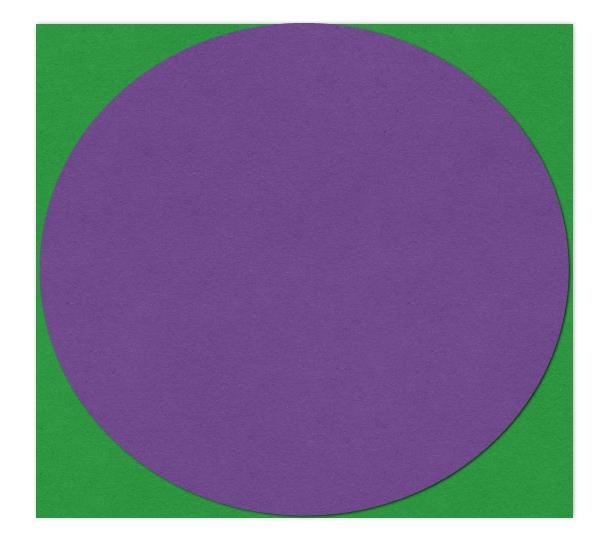
\includegraphics[width=0.50000\textwidth]{solution 1.jpg}\\
According to the picture, we can randomly choose points from the square
with area of 1and see how many points will be in the circle within the
square.

\[p = \frac{\pi}{4}\]

In such case, we will have code like this:

\begin{Shaded}
\begin{Highlighting}[]
\KeywordTok{set.seed}\NormalTok{(}\DecValTok{676}\NormalTok{)}
\NormalTok{n<-}\DecValTok{10000}
\NormalTok{count<-}\DecValTok{0}
\ControlFlowTok{for}\NormalTok{ (i }\ControlFlowTok{in} \DecValTok{1}\OperatorTok{:}\NormalTok{n)\{}
\NormalTok{  point<-}\KeywordTok{runif}\NormalTok{(}\DecValTok{2}\NormalTok{,}\OperatorTok{-}\DecValTok{1}\NormalTok{,}\DecValTok{1}\NormalTok{)}
  \ControlFlowTok{if}\NormalTok{ (point[}\DecValTok{1}\NormalTok{]}\OperatorTok{**}\DecValTok{2}\OperatorTok{+}\NormalTok{point[}\DecValTok{2}\NormalTok{]}\OperatorTok{**}\DecValTok{2} \OperatorTok{<=}\StringTok{ }\DecValTok{1}\NormalTok{)\{}
\NormalTok{    count<-count}\OperatorTok{+}\DecValTok{1}
\NormalTok{  \}}
\NormalTok{\}}
\NormalTok{spi<-count}\OperatorTok{*}\DecValTok{4}\OperatorTok{/}\NormalTok{n}
\KeywordTok{cat}\NormalTok{(}\StringTok{"}\CharTok{\textbackslash{}n}\StringTok{Our estimate of the expected pi is "}\NormalTok{,spi)}
\end{Highlighting}
\end{Shaded}

\begin{verbatim}
## 
## Our estimate of the expected pi is  3.1484
\end{verbatim}

\subsection{Solution 2: Buffon's
needles}\label{solution-2-buffons-needles}

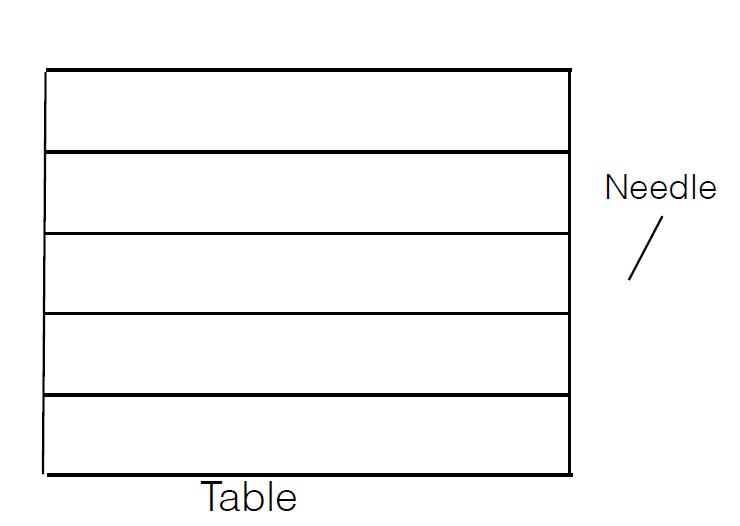
\includegraphics[width=0.50000\textwidth]{solution 2.jpg}\\
Suppose we have a floor made of parallel strips of wood, each the same
width, and we drop a needle onto the floor. What is the probability that
the needle will lie across a line between two strips?

Suppose the length of needle is \(l\), the distances between two strips
is \(t\).

Let \(x\) be the distance from the center of the needle to the closest
line, and let \(\theta\) be the acute angle between the needle and the
projected line with length \(x\).

The uniform probability density function of \(x\) between \(\theta\) and
\(\frac{t}{2}\) is:

\[\left\{  
             \begin{array}{ll}  
             \dfrac{2}{t} : 0 \le x \le \dfrac{t}{2}\\  
             0: elsewhere
             \end{array}  
\right. \]

The uniform probability density function of \(\theta\) between 0 and
\(\frac{\pi}{2}\) is:

\[\left\{
            \begin{array}{ll}
            \dfrac{2}{\pi}: 0 \le \theta \le \dfrac{\pi}{2}\\
            0:elsewhere
            \end{array}
\right.\]

In such case, the joint probability density function is the product of
these two probability density function:

\[\left\{
            \begin{array}{ll}
            \dfrac{4}{t \pi}: 0 \le x \le \dfrac{t}{2}; 0 \le \theta \le \dfrac{\pi}{2}\\
            0:elsewhere
            \end{array}
\right.\]

The needls crosses a line if:

\[x \le \frac{l}{2} cos\theta\]

In such case, we have two rules:

\begin{enumerate}
\def\labelenumi{(\arabic{enumi})}
\item
  We can set an area with width \(t\), and randomly select points in
  this area.
\item
  The probability is not related to horizontal coordinate of the point.
\end{enumerate}

Here we will have two situations:

\subsubsection{Situation 1: Short
needle}\label{situation-1-short-needle}

if \(l < t\):

\[p = \int_{\theta = 0}^\frac{\pi}{2} \int_{x = 0}^{\frac{l}{2}cos\theta} \frac{4}{t \pi} dx d\theta = \frac{2l}{t \pi}\]

In such case, we will have \(\pi\) like this:

\[\pi = \frac{2l}{tp}\]

In this situation, we will have code like this:

\begin{Shaded}
\begin{Highlighting}[]
\KeywordTok{set.seed}\NormalTok{(}\DecValTok{676}\NormalTok{)}
\NormalTok{l <-}\StringTok{ }\FloatTok{0.5}
\NormalTok{t <-}\StringTok{ }\DecValTok{1}
\NormalTok{cross <-}\StringTok{ }\KeywordTok{numeric}\NormalTok{() }\CommentTok{# whether the needle cross the line or not}
\NormalTok{numberofneedles <-}\StringTok{ }\DecValTok{1000000}

\ControlFlowTok{for}\NormalTok{ (i }\ControlFlowTok{in} \DecValTok{1}\OperatorTok{:}\NormalTok{numberofneedles)\{}
\NormalTok{  x <-}\StringTok{ }\KeywordTok{runif}\NormalTok{(}\DecValTok{1}\NormalTok{,}\DecValTok{0}\NormalTok{,t) }\CommentTok{# The vertical coordinate of the point}
\NormalTok{  theta <-}\StringTok{ }\KeywordTok{runif}\NormalTok{(}\DecValTok{1}\NormalTok{,}\DecValTok{0}\NormalTok{,pi}\OperatorTok{/}\DecValTok{2}\NormalTok{)}
  \ControlFlowTok{if}\NormalTok{ (x }\OperatorTok{<=}\StringTok{ }\NormalTok{l}\OperatorTok{/}\DecValTok{2} \OperatorTok{*}\StringTok{ }\KeywordTok{cos}\NormalTok{(theta) }\OperatorTok{|}\StringTok{ }\NormalTok{t}\OperatorTok{-}\NormalTok{x }\OperatorTok{<=}\StringTok{ }\NormalTok{l}\OperatorTok{/}\DecValTok{2} \OperatorTok{*}\StringTok{ }\KeywordTok{cos}\NormalTok{(theta))\{}
\NormalTok{    cross[i] =}\StringTok{ }\DecValTok{1}
\NormalTok{  \}}
  \ControlFlowTok{else}\NormalTok{\{}
\NormalTok{    cross[i] =}\StringTok{ }\DecValTok{0}
\NormalTok{  \}}
\NormalTok{\}}

\KeywordTok{cat}\NormalTok{(}\StringTok{"}\CharTok{\textbackslash{}n}\StringTok{The probability of a needle cross the line is"}\NormalTok{, }\KeywordTok{sum}\NormalTok{(cross)}\OperatorTok{/}\NormalTok{numberofneedles)}
\end{Highlighting}
\end{Shaded}

\begin{verbatim}
## 
## The probability of a needle cross the line is 0.318521
\end{verbatim}

\begin{Shaded}
\begin{Highlighting}[]
\NormalTok{spi2 <-}\StringTok{ }\DecValTok{2}\OperatorTok{*}\NormalTok{l}\OperatorTok{/}\NormalTok{(t }\OperatorTok{*}\StringTok{ }\KeywordTok{sum}\NormalTok{(cross) }\OperatorTok{/}\StringTok{ }\NormalTok{numberofneedles)}

\KeywordTok{cat}\NormalTok{(}\StringTok{"}\CharTok{\textbackslash{}n}\StringTok{Our estimate of the expected pi is"}\NormalTok{, spi2)}
\end{Highlighting}
\end{Shaded}

\begin{verbatim}
## 
## Our estimate of the expected pi is 3.13951
\end{verbatim}

\subsubsection{Situation 2: Long needle}\label{situation-2-long-needle}

if \(l < t\): \[ \begin{split}
&When \frac l2cos(\theta) = \frac t2, \\
&\theta = arccos(\frac tl)
\end{split}\] \[ \begin{split}
p &= \int_{\theta = 0}^\frac{\pi}{2} \int_{x = 0}^{min(\theta)} \frac{4}{t \pi} dx d\theta\ where\ min(\theta) = min(\frac t2, \frac{l}{2}cos(\theta))\\
&= \int_{\theta = 0}^{arccos(\frac tl)} \int_{x = 0}^{\frac t2} \frac{4}{t \pi} dx d\theta\ +\ \int_{\theta = arccos(\frac tl)}^{\frac{\pi}{2}} \int_{x=0}^{\frac l2 cos(\theta)} \frac{4}{t \pi} dxd \theta \\
&= \frac{2}{\pi} arccos(\frac tl)\ +\ \frac{2l}{\pi t}(1\ -\ \sqrt{1\ -\ \frac{t^2}{l^2}}) \\
\pi &= \frac 2p arccos(\frac tl) + \frac {2l}{tp} (1\ -\ \sqrt{1\ -\ \frac{t^2}{l^2}})
\end{split}\]

In such case, we will have code like this:

\begin{Shaded}
\begin{Highlighting}[]
\KeywordTok{set.seed}\NormalTok{(}\DecValTok{676}\NormalTok{)}
\NormalTok{l <-}\StringTok{ }\DecValTok{2}
\NormalTok{t <-}\StringTok{ }\DecValTok{1}
\NormalTok{cross <-}\StringTok{ }\KeywordTok{numeric}\NormalTok{() }\CommentTok{# whether the needle cross the line or not}
\NormalTok{numberofneedles <-}\StringTok{ }\DecValTok{1000000}

\ControlFlowTok{for}\NormalTok{ (i }\ControlFlowTok{in} \DecValTok{1}\OperatorTok{:}\NormalTok{numberofneedles)\{}
\NormalTok{  x <-}\StringTok{ }\KeywordTok{runif}\NormalTok{(}\DecValTok{1}\NormalTok{,}\DecValTok{0}\NormalTok{,t) }\CommentTok{# The vertical coordinate of the point}
\NormalTok{  theta <-}\StringTok{ }\KeywordTok{runif}\NormalTok{(}\DecValTok{1}\NormalTok{,}\DecValTok{0}\NormalTok{,pi}\OperatorTok{/}\DecValTok{2}\NormalTok{)}
  \ControlFlowTok{if}\NormalTok{ (x }\OperatorTok{<=}\StringTok{ }\NormalTok{l}\OperatorTok{/}\DecValTok{2} \OperatorTok{*}\StringTok{ }\KeywordTok{cos}\NormalTok{(theta) }\OperatorTok{|}\StringTok{ }\NormalTok{t}\OperatorTok{-}\NormalTok{x }\OperatorTok{<}\StringTok{ }\NormalTok{l}\OperatorTok{/}\DecValTok{2} \OperatorTok{*}\StringTok{ }\KeywordTok{cos}\NormalTok{(theta))\{}
\NormalTok{    cross[i] =}\StringTok{ }\DecValTok{1}
\NormalTok{  \}}
  \ControlFlowTok{else}\NormalTok{\{}
\NormalTok{    cross[i] =}\StringTok{ }\DecValTok{0}
\NormalTok{  \}}
\NormalTok{\}}

\NormalTok{p <-}\StringTok{ }\KeywordTok{sum}\NormalTok{(cross)}\OperatorTok{/}\NormalTok{numberofneedles}

\KeywordTok{cat}\NormalTok{(}\StringTok{"}\CharTok{\textbackslash{}n}\StringTok{The probability of a needle cross the line is"}\NormalTok{, p)}
\end{Highlighting}
\end{Shaded}

\begin{verbatim}
## 
## The probability of a needle cross the line is 0.837051
\end{verbatim}

\begin{Shaded}
\begin{Highlighting}[]
\NormalTok{spi3 <-}\StringTok{ }\DecValTok{2} \OperatorTok{/}\StringTok{ }\NormalTok{p }\OperatorTok{*}\StringTok{ }\KeywordTok{acos}\NormalTok{(t}\OperatorTok{/}\NormalTok{l) }\OperatorTok{+}\StringTok{ }\DecValTok{2}\OperatorTok{*}\NormalTok{l }\OperatorTok{/}\StringTok{ }\NormalTok{(t }\OperatorTok{*}\StringTok{ }\NormalTok{p) }\OperatorTok{*}\StringTok{ }\NormalTok{(}\DecValTok{1} \OperatorTok{-}\StringTok{ }\KeywordTok{sqrt}\NormalTok{(}\DecValTok{1} \OperatorTok{-}\StringTok{ }\NormalTok{t}\OperatorTok{^}\DecValTok{2} \OperatorTok{/}\StringTok{ }\NormalTok{l}\OperatorTok{^}\DecValTok{2}\NormalTok{))}

\KeywordTok{cat}\NormalTok{(}\StringTok{"}\CharTok{\textbackslash{}n}\StringTok{Our estimate of the expected pi is"}\NormalTok{, spi3)}
\end{Highlighting}
\end{Shaded}

\begin{verbatim}
## 
## Our estimate of the expected pi is 3.142334
\end{verbatim}

It seems that using longer needles will get the better estimation. But I
don't know if the assumption is true and how to prove it.


\end{document}
